% !TeX document-id = {1d4de9fb-623d-4c26-a748-2d875501d5b0}
% !TeX TS-program = lualatex
% !BIB TS-program = biber

\documentclass[10pt]{book}

\usepackage{iftex}

\ifPDFTeX
	\usepackage{cmap} % should be first
	\usepackage[utf8]{inputenc}
	\usepackage[T1,T2A]{fontenc}
	\usepackage[english,russian]{babel}

	\usepackage[breakwords]{truncate}
\fi

\ifLuaTeX
	\usepackage{fontspec}

	% from https://github.com/AndreyAkinshin/Russian-Phd-LaTeX-Dissertation-Template/
	\setmonofont{CMU Typewriter Text}
	\newfontfamily\cyrillicfonttt{CMU Typewriter Text}
	\defaultfontfeatures{Ligatures=TeX}
	\setmainfont{CMU Serif}
	\newfontfamily\cyrillicfont{CMU Serif}
	\setsansfont{CMU Sans Serif}
	\newfontfamily\cyrillicfontsf{CMU Sans Serif}
	
	\usepackage{polyglossia}
	\setmainlanguage[babelshorthands=true]{russian}
	\setotherlanguage{english}
%	\setotherlanguage{german}
	
	\usepackage[fit]{lualatex-truncate}
\fi

% Programming
\usepackage{xifthen}

% Language support

\usepackage{csquotes}

% Typesetting
\usepackage{enumitem}
\usepackage{indentfirst}
\usepackage{titlesec}
%\usepackage{tocbibind}
\usepackage{xspace}
\usepackage{setspace}
\onehalfspacing

% Extra symbols
\usepackage{fontawesome5}
\usepackage{textcomp}

% Tables
\usepackage{array}
\usepackage{booktabs}

% Highlightiing
\usepackage[normalem]{ulem}

% Math
\usepackage{amsmath}
\usepackage{amssymb}
\usepackage{commath}
\newcommand{\vect}[1]{\mathbf{#1}}
\DeclareMathOperator{\const}{const}




%%% Drawing with TikZ / pgfplots
\usepackage{graphicx}

\usepackage[svgnames,x11names]{xcolor}
\colorlet{tabblue}{blue!70!green}
\colorlet{tabgreen}{green!50!black!85!white}
\colorlet{taborange}{orange}
\colorlet{tabred}{red!80!black}

\usepackage{tikz}
\usetikzlibrary{arrows.meta}
\usetikzlibrary{bbox}
\usetikzlibrary{calc}
\usetikzlibrary{decorations.markings}
\usetikzlibrary{decorations.pathmorphing}
\usetikzlibrary{decorations.pathreplacing}
\usetikzlibrary{external}
\usetikzlibrary{fadings}
\usetikzlibrary{math}
\usetikzlibrary{matrix}
\usetikzlibrary{patterns}
\usetikzlibrary{positioning}
\usetikzlibrary{shapes.geometric}
\usetikzlibrary{shapes.misc}


%%% PGFplots setup
\usepackage{pgfplots}
\usepackage{pgfplotstable}

\newcommand{\tickprint}[1]{\small\pgfmathprintnumber[verbatim,#1]{\tick}}

\pgfplotsset{
	compat=newest,
	xticklabel=\tickprint{},
	yticklabel=\tickprint{},
	scaled y ticks=false,
	%	set layers=axis on top, % BAD!
	every axis/.append style={
		line width=0.6pt, % /tikz/semithick==0.6pt
		%
		scaled y ticks=false,
		ticklabel shift=0pt,
		tick align=inside,
		tick pos=left,
		tickwidth=0.6pt,
		subtickwidth=0.6pt,
		major tick length=3pt,
		minor tick length=1.5pt,
		tick style={semithick,black,overlay},
		%
		minor tick num=4,
	},
}






%%% TikZ helpers (for debug purposes)
\tikzset{nosep/.style={inner sep=0,outer sep=0}}

\newcommand{\helpangles}[1]{
	\foreach \a in {0,5,...,355} \draw[help lines] (#1.center) -- (#1.\a) -- ++(\a:0.5) node[font=\tiny] {\a};
}

\tikzset{%
	show curve controls/.style={
		postaction={
			decoration={
				show path construction,
				curveto code={
					\draw [blue,very thin]
					(\tikzinputsegmentfirst) -- (\tikzinputsegmentsupporta)
					(\tikzinputsegmentlast) -- (\tikzinputsegmentsupportb);
					\fill [red, opacity=0.5]
					(\tikzinputsegmentsupporta) circle [radius=.5ex]
					(\tikzinputsegmentsupportb) circle [radius=.5ex];
				}
			},
			decorate
}}}
\tikzset{show curve controls/.style={}}  % disables code above




% Hyperlinks
\usepackage{hyperref}  % should be last
\hypersetup{
	linktocpage,
	colorlinks,
	linkcolor={red!70!black},
	citecolor={green!50!black},
	urlcolor={blue!80!black}
}
\newcommand*{\email}[1]{\href{mailto:#1}{\nolinkurl{#1}} } 


%%% Colorful fixmes and missing refs and missing cites (if no biblatex is present)
% !TeX root = phd_thesis_Syromyatnikov.tex

% MUST GO AFTER \usepackage{hyperref}

% makes fixes colorful
\usepackage{fixme}
\usepackage{soulutf8}
\usepackage{etoolbox}

\ifLuaTeX
	% https://tex.stackexchange.com/questions/339382/soul-highlight-removes-some-characters-from-text
	\makeatletter
	\font\SOUL@tt="CMU Typewriter Text"
	\setbox\z@\hbox{\SOUL@tt-}
	\SOUL@ttwidth\wd\z@ %reset default width of -
	\makeatother
\fi

\fxsetup{status=draft,author= ,layout=inline,nomargin,theme=color}
\definecolor{fxnote}{rgb}{0,0,0}
\definecolor{fxwarning}{rgb}{0,0,0}
\definecolor{fxerror}{rgb}{0,0,0}
\definecolor{fxfatal}{rgb}{0,0,0}

\colorlet{fxnotebg}{green!60}
\colorlet{fxwarningbg}{yellow!60}
\colorlet{fxerrorbg}{red!40!orange!50}
\colorlet{fxfatalbg}{red!70}
% redefine the layout macro:
\makeatletter
\renewcommand*\FXLayoutInline[3]{%
    \@fxdocolon {#3}{%
        \@fxuseface {inline}%
        \begingroup
        \sethlcolor{fx#1bg}%
        \color{fx#1}\ignorespaces \hl{#3\@fxcolon #2}%
        \endgroup}}

\renewcommand*\FXLayoutContentsLine[3]{%
    \iffx@mode@multiuser%
    \fxaddcontentsline{\ignorespaces#3 \protect\sethlcolor{fx#1bg}\color{fx#1}\hl{\fxnotename{#1}:\thesection #2}}%
    \else%
    \fxaddcontentsline{\protect\sethlcolor{fx#1bg}\color{fx#1}\hl{%
    	\fxnotename{#1}:~\texttt{\thesection}~#2%
    }}%
    \fi}
\makeatother


% emphasizes missing references and citations
\makeatletter
\patchcmd{\@setref}{\bfseries ??}{\fxerror{Ref}}{}{}
\patchcmd{\@citex}{\bfseries ?}{\fxerror{Cite}}{}{}
\patchcmd{\NAT@citexnum}{\reset@font\bfseries?}{\fxerror{Cite}}{}{}
\patchcmd{\NAT@citex}{\reset@font\bfseries ?}{\fxerror{Cite}}{}{}
\makeatother
  % must go after hyperref




%%% Bibliography
\usepackage[backend=biber,
clearlang=true,autolang=other,language=autobib,
style=nature,
doi=false,url=false,eprint=false,isbn=false,
sorting=none,sortcites=true,
maxnames=7,minnames=3,defernumbers=true,date=year]{biblatex}

\addbibresource{bib/litreview.bib}
\addbibresource{bib/methods.bib}
\addbibresource{bib/interaction.bib}
\addbibresource{bib/formation.bib}
\addbibresource{bib/eqnoneq.bib}
\addbibresource{bib/spt.bib}

\addbibresource{bib/2020-review.bib}
\addbibresource{bib/master-diploma.bib}

\addbibresource{bib/articles.bib}
\addbibresource{bib/conferences.bib}

\AtEveryBibitem{
	\clearfield{issn}
	\clearfield{issue}
	\clearfield{month}
	\clearfield{abstract}
	\clearlist{language}
}

%\renewcommand{\finalnamedelim}{\addcomma\space\bibstring{and}\space}
\renewcommand{\finalnamedelim}{\addcomma\space}

\renewcommand{\bibrangedash}{\textendash}


%%% Git version
\usepackage{shellesc}
%\ShellEscape{git describe --tags --always --abbrev=40 --dirty > git-version.tex}
\ShellEscape{git describe --always --abbrev=40 --always > git-version-commit.tex}
\ShellEscape{git describe --tags --abbrev=10 --always > git-describe.tex}

\usepackage{catchfile}
%\CatchFileDef{\GitVersion}{git-version.tex}{}
\CatchFileDef{\GitCommit}{git-version-commit.tex}{}
\CatchFileDef{\GitDescribe}{git-describe.tex}{}
\hypersetup{pdfinfo={GitVersion={\GitDescribe},GitCommit={\GitCommit}}}
\usepackage[useregional]{datetime2}




%%% Technical stuff
\usepackage[figure,table,xspace]{totalcount} % count figures and tables

\usepackage{lastpage} % count pages
\usepackage{refcount}

\usepackage{totcount} % count bibliography items
\newtotcounter{phdthesiscitenum}
\setcounter{phdthesiscitenum}{-21} 
% 21 = 10 articles + 11 abstracts
\AtEveryBibitem{\stepcounter{phdthesiscitenum}}

\usepackage{lipsum}


%%% Footnote without number
\newcommand\blindfootnote[1]{%
	\begingroup
	\renewcommand\thefootnote{}\footnote{#1}%
	\addtocounter{footnote}{-1}%
	\endgroup
}


%%% Further tweaking
\renewcommand{\arraystretch}{1.2} % more vertical space in tables

% \overfullrule=2mm % shows overfull markers without 'draft' option


% titlesec
\titleformat{\chapter}[display]{\centering\large\bfseries\scshape}{}{1em minus 1em}{}[]
\titlespacing{\chapter}{0cm}{-0.5cm}{*1}[0pt]

\titleformat{\section}[runin]{\normalsize\bfseries}{}{1em minus 1em}{\uline}[\uline.]
\titlespacing{\section}{0cm}{0.3cm}{*1}[0pt]

%\titleformat{command}[shape]{format}{label}{sep}{before-code}[after-code]
%\titlespacing{command}{left}{before-sep}{after-sep}

% makes chapter able to open on any page
\usepackage{etoolbox}
\makeatletter
\patchcmd{\chapter}{\if@openright\cleardoublepage\else\clearpage\fi}{\par}{}{}
\makeatother

\usepackage{geometry}
\geometry{
	a5paper,
	top=1.5cm, inner=1.5cm,	outer=1.5cm, bottom=2cm
}



%%% Page headers / footers
\usepackage{fancyhdr}
\pagestyle{fancy}
\fancyhf{}
\fancyfoot[C]{\thepage}
\renewcommand{\headrulewidth}{0pt}
\renewcommand{\footrulewidth}{0pt}


\usepackage[font={stretch=0.90},labelfont={bf,sc},figurewithin=none]{caption}


\tikzexternalize[prefix=tikzfigures-ar/] % we want different folders for thesis and autoreferat

% очень грязный хак, меняющий & на and между последним и предпоследним авторами в списке литературы
%\AtBeginBibliography{%
%	\renewcommand*{\finalnamedelim}{%
%		\ifnumgreater{\value{liststop}}{2}{\finalandcomma}{}%
%		\addspace{and}\space}%
%}

\hypersetup{urlcolor = black}

\usepackage{chngcntr}
\counterwithout{equation}{chapter} % remove the chapter number

\begin{document}  %%%%%%%%%%%%%%%%%%%%%%%%%%%%%%%%%%%%%%%%%%%%%%%%%%%%%%%%
\thispagestyle{empty}

\begin{titlepage}
\centering
\textsc{\Large Московский государственный университет имени М.~В.~Ломоносова}

\vspace*{1cm}
\hfill \textit{На правах рукописи } \\
\vspace*{2cm}
\textsc{\bfseries Сыромятников Алексей Геральдович }\\
\rule{0cm}{1.2cm}
\begin{spacing}{1.6}
{\Large \bfseries \uppercase{Теоретическое исследование процессов формирования и структурных свойств металлических атомных проводов}}\\
\end{spacing}
\vspace*{1cm}
\begin{tabular}{ll}
Специальность  & \texttt{01.04.07} --- физика конденсированного состояния \\
\end{tabular}

\vspace*{3cm}
{\large \scshape \uppercase{автореферат}} \\
диссертации на соискание ученой степени \\
кандидата физико--математических наук \\
\vfill
Москва --- 2020

\end{titlepage}

\thispagestyle{empty} \singlespacing
\setlength{\parindent}{0cm}
Работа выполнена на кафедре общей физики физического факультета Московского государственного университета имени М. В. Ломоносова.\\

\small
\begin{tabular}{@{}p{0.37\linewidth} p{0.6\linewidth}@{}}
	\textbf{Научный руководитель} & 		\textsc{Клавсюк Андрей Леонидович}, \newline 
											кандидат физико-математических наук, доцент,
											МГУ имени М. В. Ломоносова, Физический факультет, кафедра общей физики, доцент. \\
	
	\textbf{Официальные оппоненты:} & 		\textsc{Таюрский Дмитрий Альбертович}, \newline
											доктор физико-математических наук, профессор,
											Казанский федеральный университет, заведующий кафедрой общей физики; \\
	% https://kpfu.ru/sveden/struct/prorektory/tajurskij-dmitrij-albertovich/biografiya
	
	&                           			\textsc{Кузаков Константин Алексеевич}, \newline 
											доктор физико-математических наук, доцент, 
											МГУ имени М. В. Ломоносова, Физический факультет, кафедра физики атомного ядра и квантовой теории столкновений, профессор; \\ 
	% https://istina.msu.ru/profile/kouzakov/
	
	&                           			\textsc{Гайнуллин Иван Камилевич}, \newline 
											кандидат физико-математических наук, доцент, 
											МГУ имени М. В. Ломоносова, Физический факультет, кафедра физической электроники, доцент. \\ 
	% https://istina.msu.ru/profile/Ivan.Gainullin/
\end{tabular}
\normalsize 
\vspace*{0.5cm}

Защита состоится 22 октября 2020~г. в 17 час. 00 мин. 
на заседании диссертационного совета МГУ.01.01 Московского государственного университета имени М.~В.~Ломоносова по адресу: \\
119991, Москва, ГСП-1, Ленинские горы, д.~1, стр.~2, МГУ, Физический Факультет, ауд. \underline{\hspace*{1cm}} \\

E-mail: \email{laptin@polly.phys.msu.ru} \\


С диссертацией можно ознакомиться в отделе диссертаций научной библиотеки МГУ имени М.~В.~Ломоносова (Ломоносовский просп., д.~27) и на сайте ИАС~ИСТИНА \\
\url{https://istina.msu.ru/dissertations/317745379/}
\vspace*{0.5cm}

Автореферат разослан <<~\underline{\hspace*{0.7cm}}~>> сентября 2020 года.
\vfill

Ученый секретарь \hfill %\includegraphics[width=3.6cm]{laptin-bw.jpg} \\
Диссертационного совета МГУ.01.01 \\
кандидат физико--математических наук \hfill Т.~В.~Лаптинская



\setlength{\parindent}{1em} \onehalfspacing
\newpage

\chapter{Общая характеристика работы}

\section{Актуальность темы}
Научно-технологический прогресс в настоящее время неотделим от постоянной миниатюризации различных электронных устройств, в частности интегральных микросхем и элементов памяти.
Новейшие устройства такого типа строятся на базе наноразмерных электронных компонентов, среди которых транзисторы, цепочки и провода. 
Характерные линейные размеры таких объектов сегодня приближаются к единицам нанометров. Оперировать атомными структурами такого размера очень трудно.
Поэтому прикладные и фундаментальные исследования в этой области сейчас актуальны как никогда.

Помимо этого одномерные наноструктуры обладают рядом уникальных свойств, среди которых волны спиновой и зарядовой плотности~\cite{Erwin2010}, квантованная проводимость~\cite{Klavsyuk2015}, эффект Рашбы~\cite{Rasba84.1}.
Свойства таких одномерных структур существенно отличаются как от свойств объемного образца, так и от свойств тонких пленок и квантовых точек.
Создание наноразмерных структур на текущий момент возможно либо при помощи литографических методов, либо путем перетаскивания отдельных атомов иглой сканирующего туннельного микроскопа.
Оба подхода имеют свои недостатки, не позволяющие получать такие одномерные наноструктуры в промышленных масштабах.
Ситуация может измениться с использованием метода самоорганизации наноструктур путем эпитаксиального роста.
Однако для того, чтобы использование наноструктур в промышленности стало реальностью, необходимо уметь управлять их созданием, что невозможно без понимания механизмов, ответственных за их рост.

В связи с этим особенно актуальны исследования структурных, электронных и магнитных свойств наноструктур на поверхности металлов, а также установление закономерностей в их росте и эволюции.





\section{Цель и задачи работы}
Основной целью диссертационной работы являются исследование механизмов роста атомных структур на поверхности металлов и установление особенностей их атомной структуры с использованием современных теоретических методов. Исследование механизмов роста включает в себя не только моделирование процессов самоорганизации, но и исследование взаимодействия атомов $3d$-металлов на поверхностях металлов. Для достижения поставленной цели решались следующие задачи:
\begin{enumerate}
	\item Разработать методику теоретического исследования и моделирования  формирования и дальнейшей эволюции одномерных атомных структур на поверхности металлов.
	\item Исследовать взаимодействие адатомов $3d$-металлов со ступенью вицинальной поверхности меди.
	\item Определить превалирующие факторы, влияющие на рост одномерных наноструктур на вицинальных металлических поверхностях.
	\item Показать зависимость формы распределения длин атомных цепочек от параметров эксперимента.
	\item Создать модель, описывающую распределение одномерных атомных структур, учитывающую созревание Оствальда и распад коротких одномерных структур.
	\item Исследовать структурный фазовый переход из димеризованного в недимеризованное состояние у атомных цепочек кобальта.
\end{enumerate}

Поставленные задачи важны как с фундаментальной, так и с практической точки зрения.

\section{Научная новизна работы}

В диссертационной работе получены следующие научные результаты:
\begin{enumerate}
	\item На основе метода Монте-Карло разработана методика численного моделирования формирования и эволюции морфологии одномерных металлических структур на вицинальных металлических поверхностях, а также исследован структурный фазовый переход в них.
	\item Определены особенности взаимодействия адатомов $3d$-металлов со ступенью вицинальной поверхности меди и объяснена их природа. Установлена зависимость взаимодействия между двумя адатомами $3d$-металлов на вицинальной поверхности меди от расстояния до ступени.
	\item Впервые исследован рост и последующая эволюция одномерных атомных структур при двухтемпературном режиме.
	\item Выявлена зависимость формы распределения длин атомных цепочек от таких параметров эксперимента, как температура, поток напыляемых атомов, степень покрытия.
	\item Впервые предложен метод более точного определения значения энергии связи в одномерных атомных структурах.
	\item Установлена зависимость температуры структурного фазового перехода от длины цепочки  и от энергии димеризации.
\end{enumerate}




\section{Научная и практическая значимость работы}
Полученные результаты могут иметь важное значение в решении прикладных задач по созданию новых методик производства элементов памяти и передачи информации в промышленности. Кроме того, модели описания роста одномерных структур необходимы для более корректного анализа экспериментальных данных.

Работа была  выполнена при финансовой поддержке Российского Фонда Фундаментальных Исследований (гранты 19-32-90045, 19-12-50010) и Фонда развития теоретической физики и математики ``БАЗИС''. При выполнении работы были использованы вычислительные ресурсы Научно-исследовательского вычислительного центра Московского государственного университета им. М.~В.~Ломоносова (НИВЦ МГУ).


\section{Положения, выносимые на защиту}
\begin{enumerate}
\item Метод моделирования формирования и эволюции одномерных структур на вицинальных металлических поверхностях.
\item Микроскопический механизм формирования металлических атомных проводов на вицинальных металлических поверхностях, сценарии эволюции системы атомов при различных внешних условиях.
\item Модель для описания распределения одномерных атомных структур, в рамках которой возможно более точное определение значения энергии связи.
\item Структурный фазовый переход в атомных проводах Co на поверхности Cu(775).
\end{enumerate}

\section{Достоверность результатов}
Результаты, представленные в диссертационной работе, получены с использованием  современных методов теоретической физики. Обоснованность и достоверность определяются адекватностью применяемых моделей и сравнением с экспериментальными данными.

\section{Апробация результатов}
Основные результаты диссертации были представлены автором лично на следующих мероприятиях:
\begin{itemize}[nosep]
\item VIII Всероссийская научная молодежная школа-конференция ``Химия, физика, биология: пути интеграции'' (Москва, Россия, 2020);
\item 8-ая Международная мастерская по магнитным проводам IWMW-2019 (Светлогорск, Россия, 2019);
\item III Международная Балтийская конференция по магнетизму IBCM-2019 (Светлогорск, Россия, 2019);
\item Международная конференция по нанонауке и технологии ICN+T (Брно, Чехия, 2018);
\item VI Научная молодежная школа-конференция ``Химия, физика, биология: пути интеграции'' (Москва, Россия, 2018);
\item V Научная молодежная школа-конференция ``Химия, физика, биология: пути интеграции'' (с. Ершово, Московская обл., Россия, 2017);
\item 32-я Европейская конференция физики поверхности ECOSS-32 (Гренобль, Франция, 2016);
\item 23-я Международная научная конференция студентов, аспирантов и молодых ученых ``Ломоносов-2016'' (Москва, Россия, 2016);
\item 22-я Международная научная конференция студентов, аспирантов и молодых ученых ``Ломоносов-2015'' (Москва, Россия, 2015);
\end{itemize}

\section{Публикации}
По теме диссертации опубликовано 10 научных статей и тезисы к 11 докладам на научных конференциях (всего 21 печатная работа).

\section{Личный вклад автора}
Вклад автора в диссертационную работу является определяющим. Все основные результаты работы получены автором лично, либо при его непосредственном участии.

\section{Структура и содержание работы}
Диссертация состоит из введения, шести глав, заключения и списка литературы.
Работа изложена на 117~страницах, включает 44~рисунка и 4~таблицы. Общее число ссылок составляет 173.
Каждую главу предваряет вступительная часть, представляющая краткое содержание и основные задачи текущей главы.
В конце диссертации сформулированы основные результаты, достигнутые в ней.


\chapter{Краткое содержание работы}

Во \textbf{введении} обоснована актуальность темы диссертации, указана ее научная новизна и практическая значимость, приведено краткое содержание работы по главам.

В \textbf{первой главе} приводится обзор литературы по теме диссертации. В ней проанализированы теоретические и экспериментальные работы, в которых представлены исследования свойств атомных структур, в том числе одномерных, на поверхности металлов. В частности, дан обзор  работ, посвященных росту наноструктур кобальта на вицинальной поверхности меди. Проанализированы ранее полученные распределения длин одномерных наноструктур на ступенчатых поверхностях и подходы к их получению.
Описан эксперимент, в котором впервые было показано наличие двух структурных фаз у кобальтовой проволоки на поверхности меди.

Во \textbf{второй главе} представлено описание методов моделирования наноструктур, использованных в данной работе, а именно теории функционала плотности и методов Монте-Карло, в частности алгоритма Метрополиса и кинетического метода Монте-Карло.

В \textbf{третьей главе} рассматривается взаимодействие адатомов $3d$-металлов на вицинальной поверхности меди.

\begin{figure}[t]
	\centering
	\tikzsetnextfilename{mplb2016-23}
	\begin{tikzpicture}
	\node (pic) {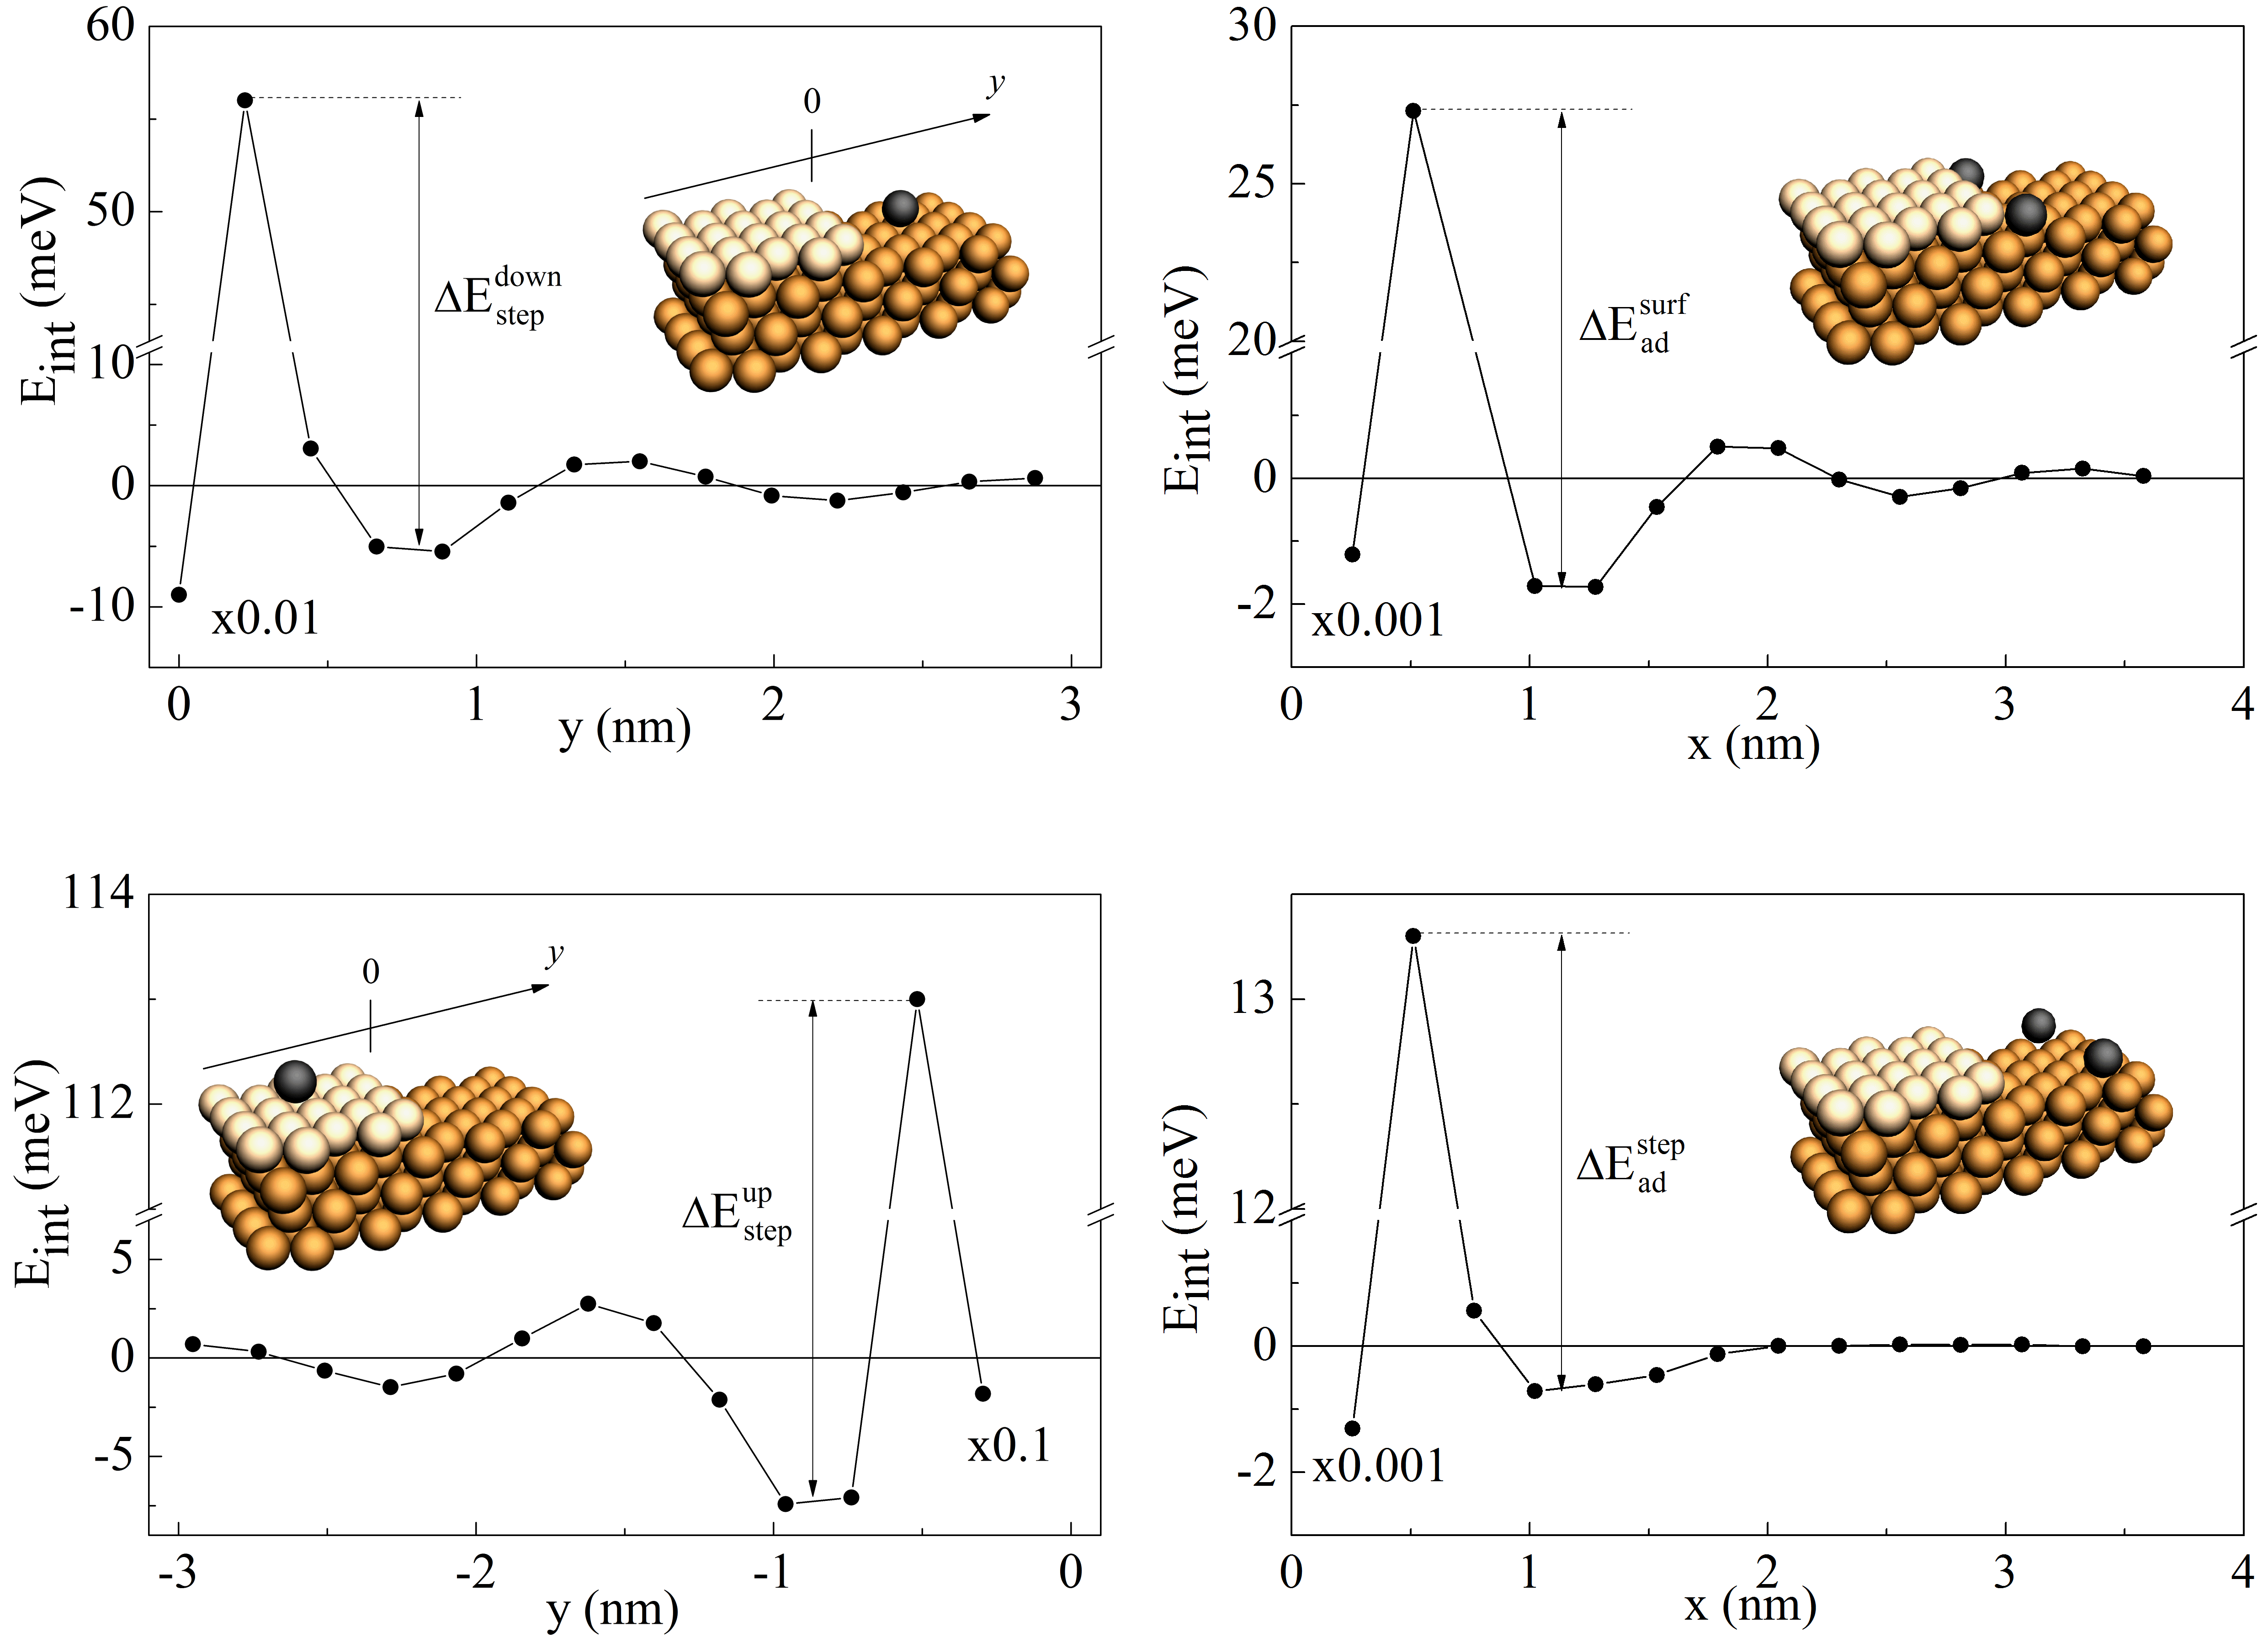
\includegraphics[width=0.95\linewidth]{fig/mplb2016/picture2+3.png}};
	\node[below left,draw] at (pic.north west) {a};
	\node[below left,draw] at (pic.184) {б};
	\node[below left,draw] at (pic.85) {в};
	\node[below left,draw] at (pic.184 -| pic.85) {г};
	\end{tikzpicture}
	\caption{
		(а, б) Взаимодействие между адатомом Ni и краем террасы вицинальной поверхности Cu(111) (а) снизу и (б) сверху от края ступени. $y$~--- расстояние от края ступени. Значение первой точки масштабировано в (а) 0.01 и (б) 0.1 раз.
		(в, г) Взаимодействие между адатомами Ni (в) вдали и (г) вблизи от края ступени. $x$~--- расстояние между адатомами. Значение первой точки масштабировано в 0.001 раз.}
	\label{fig:mplb2016-23}
\end{figure}

В первом параграфе третьей главы описывается взаимодействие адатомов со ступенью и между собой в случае бесконечно широких террас. Взаимодействие адатомов между собой и со ступенью является суперпозицией нескольких видов взаимодействий: прямого, диполь-дипольного и взаимодействия, осуществляемого через электронный газ ступени. Предложена полуэмпирическая модель, позволяющая рассчитывать энергию взаимодействия адатомов между собой и со ступенью. Именно диполь-дипольное взаимодействие, возникающее из-за перераспределения электрического заряда вблизи ступени, и фриделевское электростатическое взаимодействие объясняют отталкивающий барьер ступени.
Результаты, полученные в рамках предложенной модели, были проверены при помощи квантовомеханических расчетов методом функций Грина Корринги-Кона-Ростокера в приближении локальной спиновой плотности.

Представленные результаты объясняют предпочтение роста одномерных атомных структур на нижней террасе вместо верхней. Различие в отталкивающих барьерах для адатома Co со ступенью может приводить к тому, что при низких температурах адатомы Co будут приближаться к ступени снизу и, как следствие, формировать структуры там. Была проведена оценка частоты подхода атомов к краю ступени снизу и сверху.

Помимо этого была рассчитана энергия взаимодействия других адатомов $3d$-металлов со ступенью, а также между собой. Взаимодействие между адатомом Ni и краем террасы вицинальной поверхности Cu(111), а также между двумя адатомами Ni представлено на рисунке~\ref{fig:mplb2016-23}.

Во втором параграфе было исследовано взаимодействие адатомов со ступенью в случае узких террас (на примере поверхности Cu(775), террасы которой состоят из 6 атомных рядов). Было продемонстрировано изменение потенциальных барьеров для прыжков адатома по поверхности в зависимости от наличия цепочки на верхней или нижней террасе. Описано явление ``наносемафора''. Карта потенциальных барьеров для адатома Co на вицинальной поверхности Cu(775) показана на рисунке~\ref{fig:potentials}.

\begin{figure}[t]
	\centering
	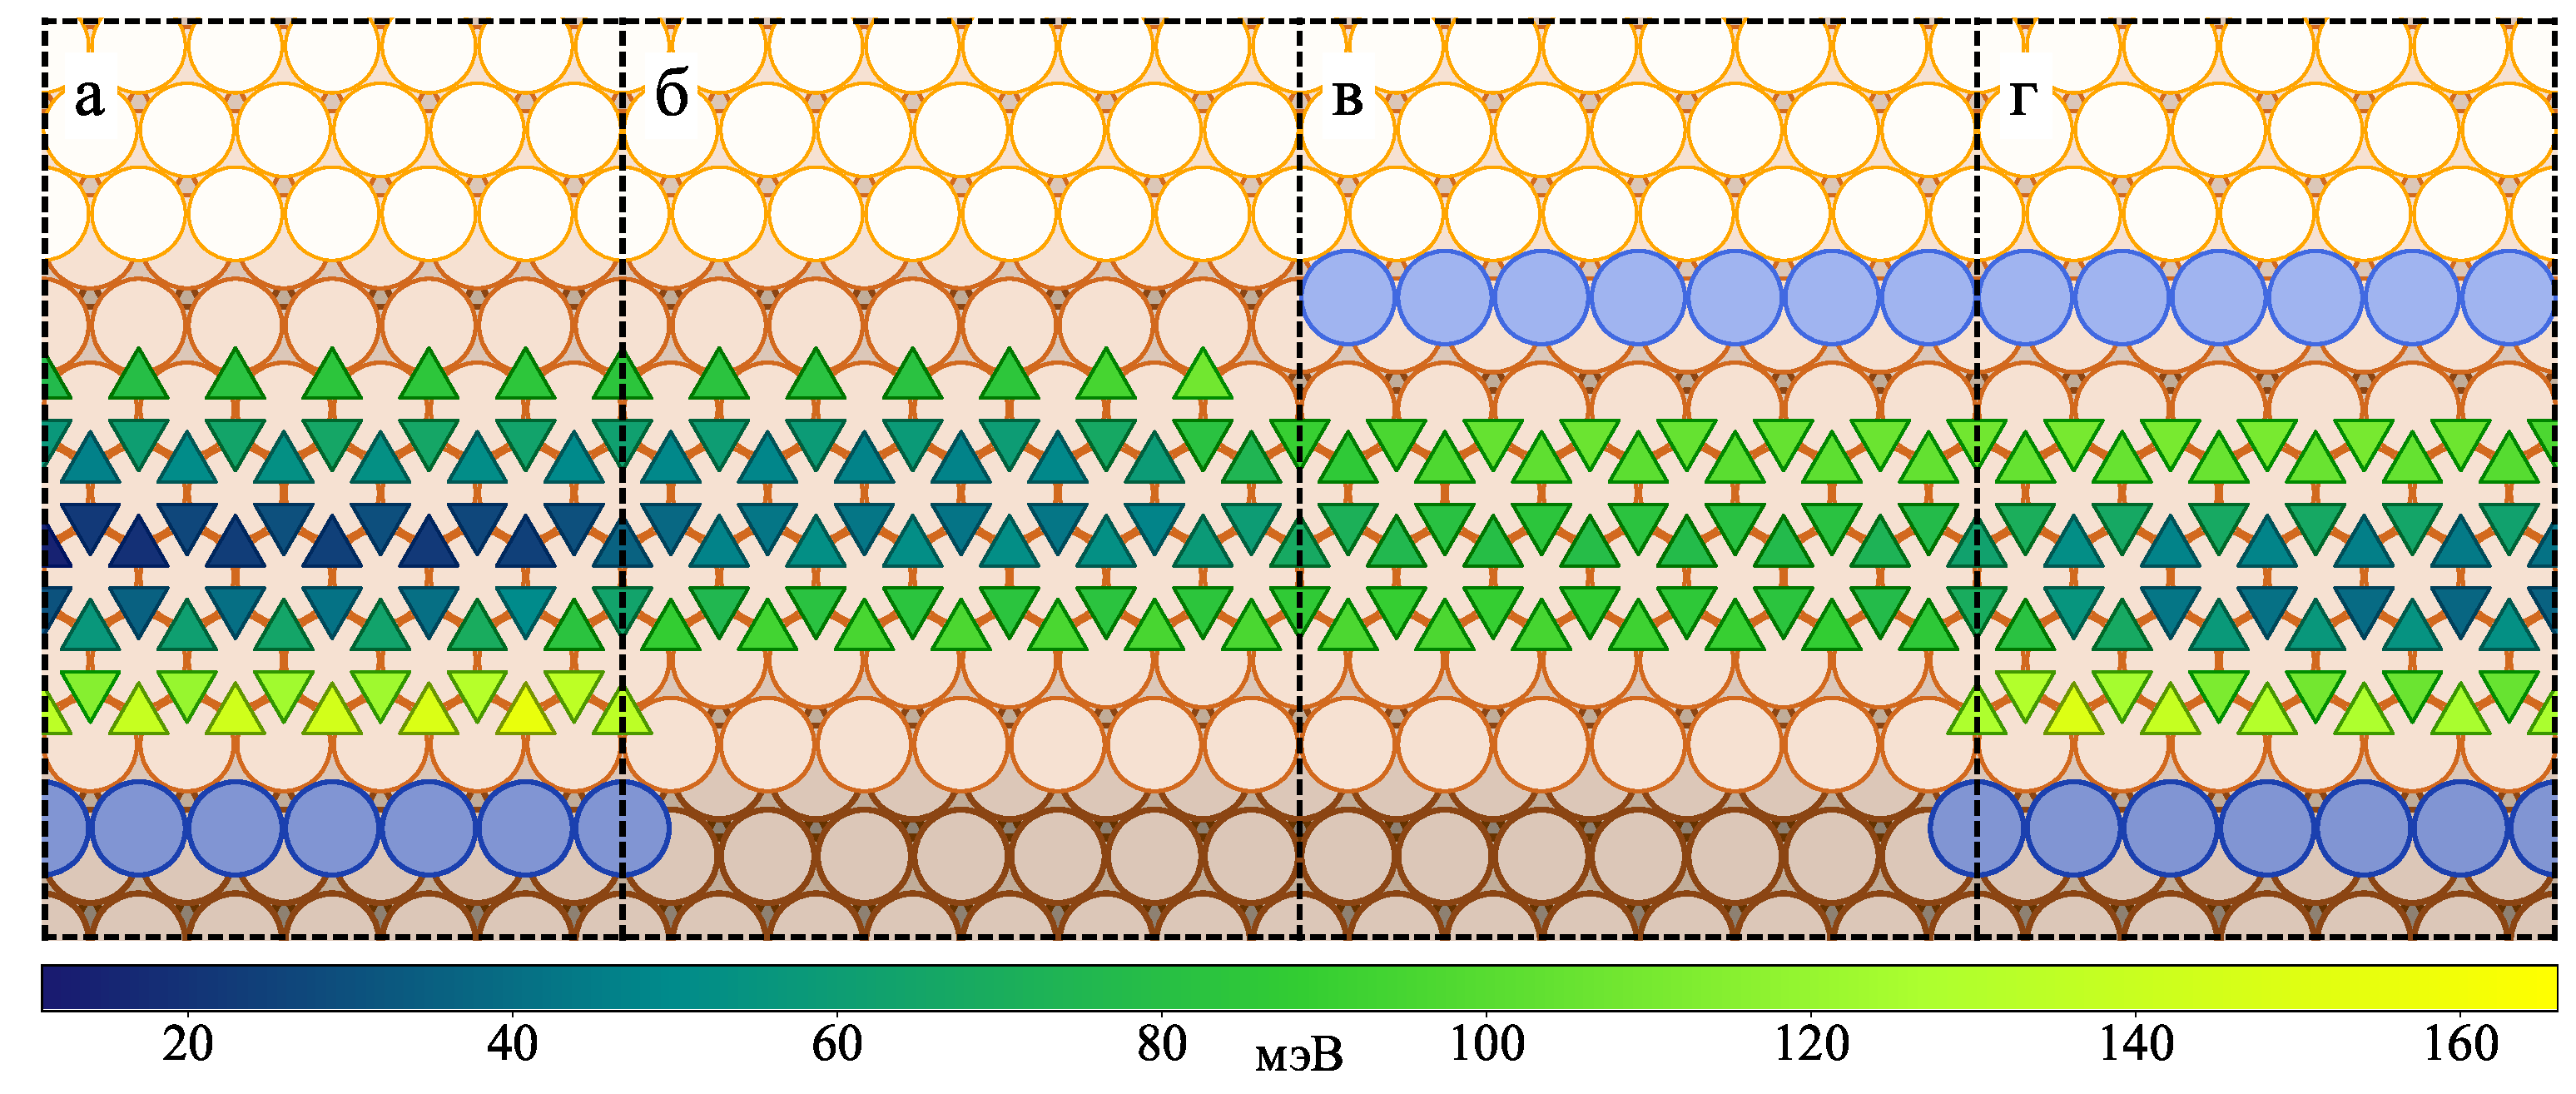
\includegraphics[width=\linewidth]{fig/map_1_h____tri-p.pdf}
	\caption{Карта потенциальной энергии для адатома Co на вицинальной поверхности Cu(775).
		(а) и (в) На поверхности присутствуют атомные цепочки кобальта на нижней или верхней террасах, соответственно.
		(б) Чистая поверхность.
		(г) На поверхности присутствуют атомные цепочки кобальта.
		Треугольниками, направленными острием вверх, обозначены ГЦК положения; направленными острием вниз --- ГПУ положения.}
	\label{fig:potentials}
\end{figure}

В третьем параграфе третьей главы показана зависимость энергии связи цепочки Co на вицинальной поверхности Cu(111). Показано, что энергия связи экспоненциальным образом убывает с ростом цепочки.



В \textbf{четвертой главе} рассматривается формирование наноструктур на вицинальных металлических поверхностях.

В первом параграфе описывается комплекс программ \texttt{kMC4}, позволяющий моделировать осаждение адатомов и последующую эволюцию образующихся наноструктур.

В следующем параграфе описываются результаты моделирования наноструктур, образующихся при росте в однотемпературном режиме. При моделировании учитываются такие эффекты, как перераспределение электрического заряда вблизи ступени, ранее описанный размерный эффект энергии связи в цепочке и созревание Оствальда. Такие параметры эксперимента, как температура, поток осаждаемых атомов, степень покрытия, брались из экспериментальных работ. Согласно полученным результатам, распределение длин цепочек получается мономодальным и хорошо описывается распределением Гаусса. Такое распределение хорошо описывает экспериментальные данные. При этом значение наиболее вероятной длины цепочки увеличивается вместе с ростом температуры образца. Помимо прочего, форма распределения сохраняется постоянной при сохранении отношения полного числа напыляемых адатомов к длине террасы при замороженных прочих параметрах.
Было показано, что при однотемпературном режиме на форму распределения оказывают влияние только изменения концентраций адатомов и/или дефектов, а также температуры.

В третьем параграфе описывается рост наноструктур на вицинальных поверхностях при двухтемпературном режиме. Такой режим описывает эксперимент, в котором осаждение происходит при одной температуре, а между ним и получением изображения происходит еще фаза отжига при другой, более высокой температуре.
Было обнаружено, что даже существенное различие во временах отжига (несколько порядков) практически не влияет на форму распределения и положение его максимума. Однако в реальном эксперименте поверхность часто неидеальна и имеет несколько характерных ширин. Учитывая этот факт, были получены распределения длин цепочек, имеющие несколько пиков, как на рисунке~\ref{fig:our_distributions_2T}. При правильном подборе ширин террас возможно получить распределения, описывающие цепочки с так называемыми ``магическими'' длинами~\cite{Mocking2013} (см. рис.~\ref{fig:our_distributions_2T}б).

\begin{figure}
	\centering
	\tikzsetnextfilename{our_distributions_2T}
	\begin{tikzpicture}
	\pgfplotsset{
		width=0.5\linewidth,
		height=4.5cm,
		xlabel={Длина, атомы},
		xmin=0, ymin=0,
		yticklabel=\tickprint{fixed,fixed zerofill,precision=2},
		%
		hist/.style={
			const plot mark mid, mark=none, fill opacity=0.5
		}
	}

	\tikzset{
		coor/.style={yshift=0.1cm},
		Z/.style={stealth-,ultra thick},
	}

	\begin{axis}[
	name=A, xmax=110, ylabel={Вероятность},
	]
	\addplot+ [hist,draw=tabblue,fill=tabblue] table[x=len,y=probab,col sep=comma] {fig/formation/2T-form-peaks/valuesA.csv} coordinate[name=X1,pos=55/132,coor];
	\end{axis}

	\begin{axis}[
	name=B, xmax=80,
	at={(A.east)}, anchor=west, xshift=1cm,
	]
	\addplot+ [hist,draw=taborange,fill=taborange] table[x=len,y=probab,col sep=comma] {fig/formation/2T-form-peaks/valuesB.csv} coordinate[name=Y1,pos=15/90,coor] coordinate[name=Y2,pos=31/90,coor];
	\end{axis}

	\draw[Z] (X1) -- ++(0, 0.7cm);
	\draw[Z] (Y1) -- ++(0, 0.7cm);
	\draw[Z] (Y2) -- ++(0, 0.7cm);

	\node[below left=0.4cm] at (A.north east) {а};
	\node[below left=0.4cm] at (B.north east) {б};
	\end{tikzpicture}
	\caption{Распределения длин атомных цепочек: напыление при температуре 160~K, отжиг при 300~K.
		(а) ширины террас слабо отличаются друг от друга,
		(б) поверхность имеет террасы с тремя характерными ширинами.
		Стрелками выделены пики, появляющиеся из-за разницы в ширинах террас.
	}
	\label{fig:our_distributions_2T}
\end{figure}

Было показано, что если после осаждения цепочки находились в состоянии термодинамического равновесия, то в процессе отжига его сменяет неравновесное состояние. По прошествии некоторого времени неравновесное состояние снова сменяется равновесным, что схематически показано
на рисунке~\ref{fig:from-eq-to-neq}. Однако часто этот процесс оказывается достаточно длительным, поэтому экспериментальный анализ длин одномерных атомных структур происходит, когда равновесное состояние еще не наступило. Это говорит о том, что не всегда можно использовать равновесные теоретические модели для определения энергии связи цепочек на поверхности.

\begin{figure}
	\centering
	\tikzsetnextfilename{from-eq-to-neq}
	\begin{tikzpicture}[x=0.71cm,y=0.71cm]%[every node/.style={scale=0.7},x=0.71cm,y=0.71cm]
	% 0.707 = 1/sqrt(2): A4 -> A5
	\node[draw,nosep,below left] (main) {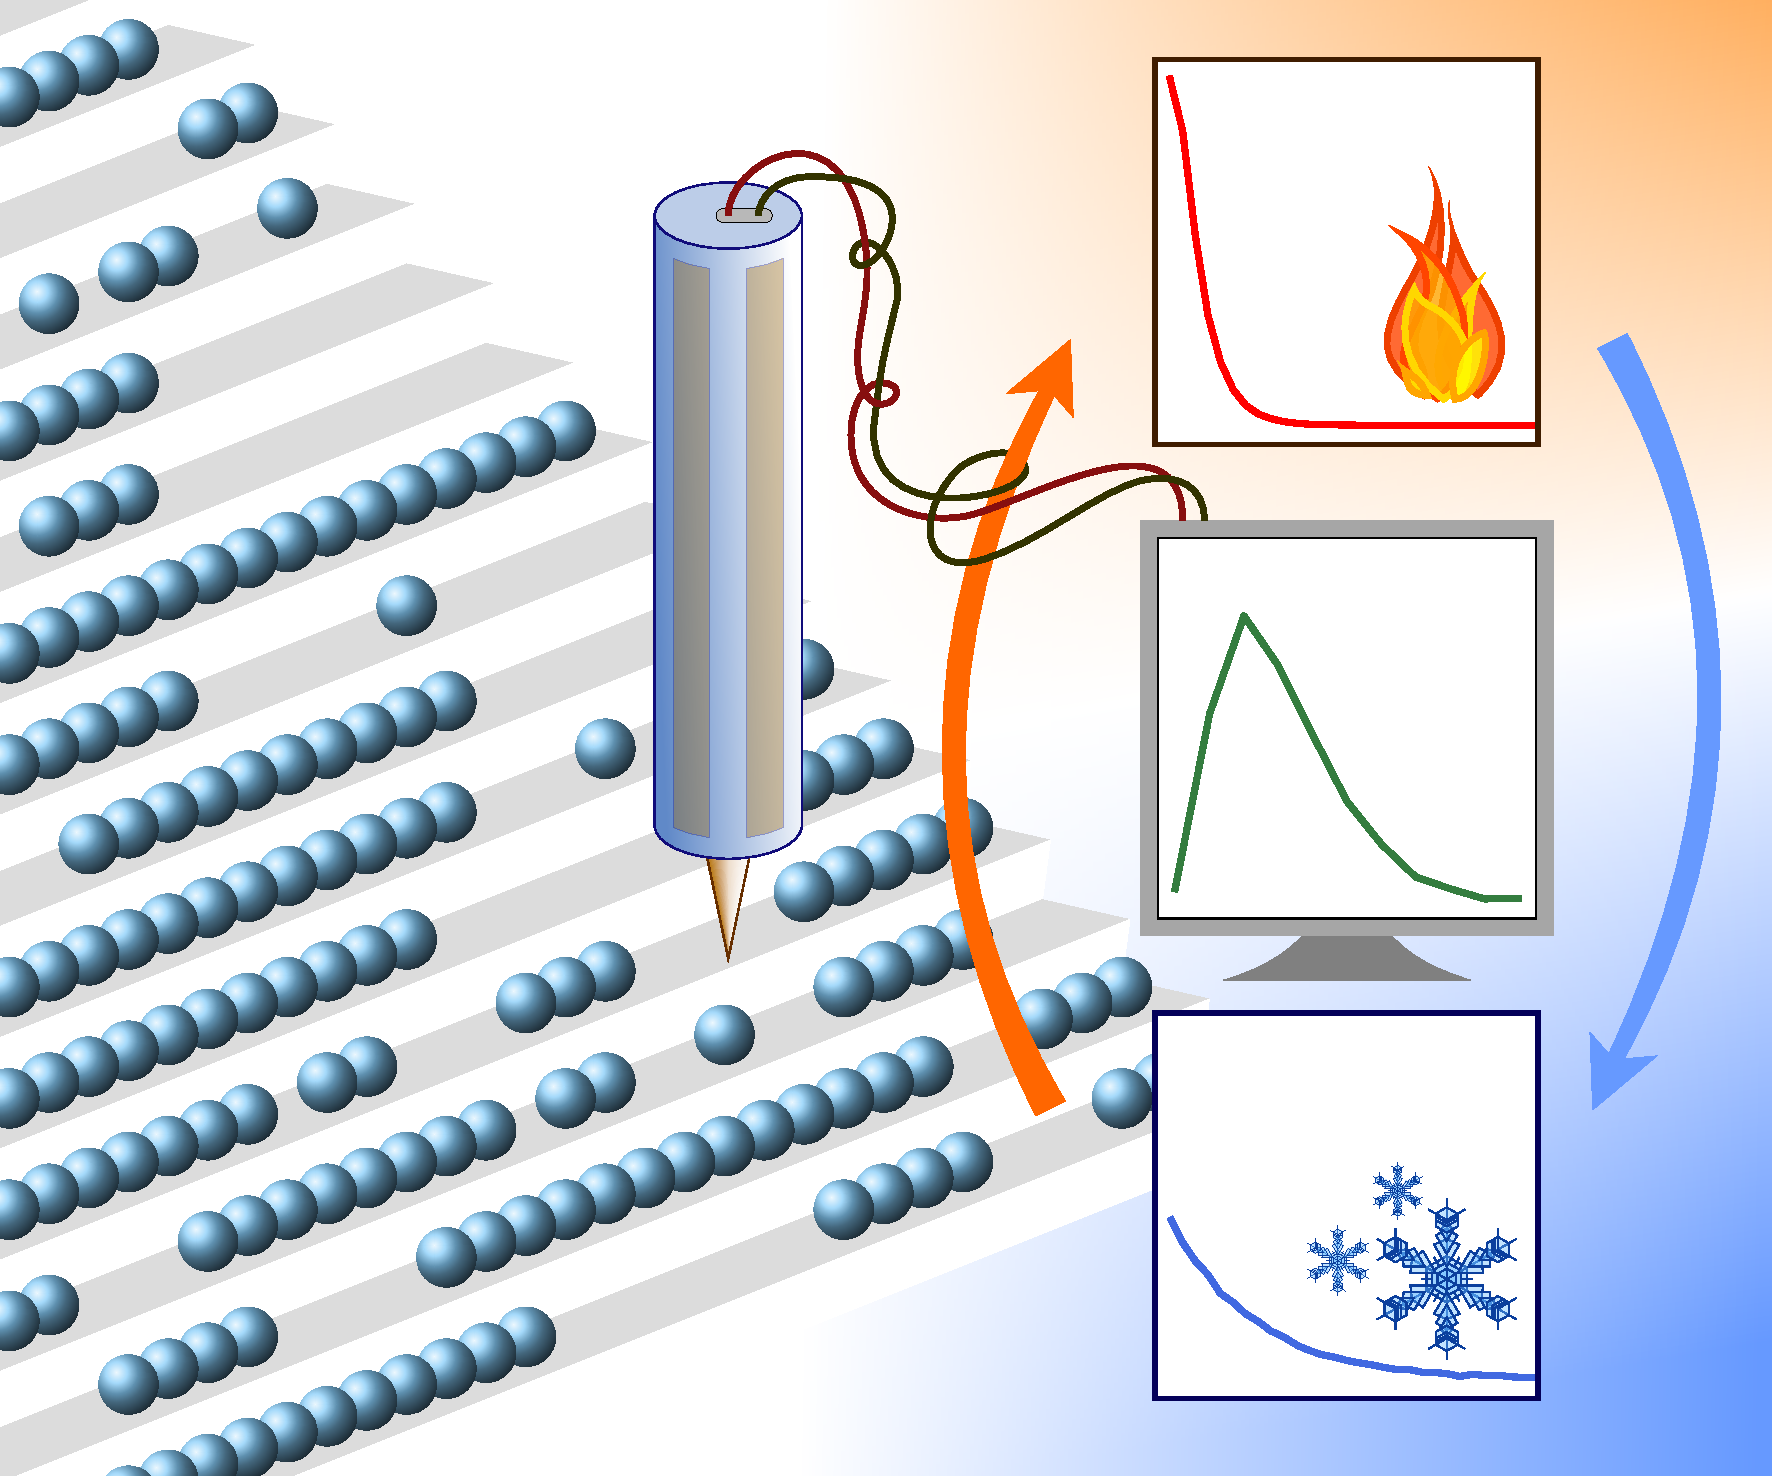
\includegraphics[width=\linewidth]{fig/Picture4-ga.pdf}};
	\begin{scope}[align=right]
	\node[below left,shift={(-2.2,-0.53)}] at (main.north east) {Равновесное\\ состояние};
	\node[below left,shift={(-2.15,-5.03)}] at (main.north east) {Неравновесное\\ состояние};
	\node[below left,shift={(-2.2,-9.47)}] at (main.north east) {Равновесное\\ состояние};
	\end{scope}
	\end{tikzpicture}
	\caption{Схематическое изображение иглы сканирующего туннельного микроскопа и неравновесного распределения длин цепочек, получаемого экспериментально, и равновесных распределений, образующихся по прошествии некоторого времени с изменением температуры.}
	\label{fig:from-eq-to-neq}
\end{figure}


В \textbf{пятой главе} обсуждаются равновесное и неравновесное распределения длин одномерных островков.

В первом параграфе выводится выражение для равновесной функции распределения длин одномерных островков. При выводе в качестве основания берется одномерная модель решеточного газа, и далее в рамках статистической физики выводится конечное выражение.
Обсуждается неявная зависимость выражения от температуры, а также функция количества островков на террасе от температуры.
Показано, что число островков растет вместе с ростом температуры и выходит на плато в пределе высоких температур, причем эта зависимость носит нелинейный характер.

В следующем параграфе обсуждаются времена жизни одномерных островков. В качестве примера берутся две системы, Ag/Pt и Co/Cu. Особый упор делается на различие потенциальных барьеров для диффузии вдоль края ступени в обеих системах и энергии связи $E_{bind}$ и на следующее отсюда различие в видах распределения длин цепочек. Система Ag/Pt может быть описана в рамках одномерной модели решеточного газа, так как в силу небольшой величины потенциальных барьеров она успевает придти к равновесию за время эксперимента. В отличие от нее система Co/Cu остается в неравновесном состоянии. Рассматривается эволюция распределения длин островков с ростом времени отжига, показано, что при этом положение максимума распределения перемещается с некоторого значения в область совсем коротких островков, то есть система приходит в термодинамически равновесное состояние.
Вводится критерий устойчивости одномерного островка, отношение к единице значения $E_{bind}/k_B T$, где $k_B$ --- постоянная Больцмана, $T$ --- температура. Если $E_{bind}/k_B T \gg 1$, то одномерный островок будет устойчивым.

В третьем параграфе выводится выражение для распределения длин одномерных островков. В процессе охлаждения переход из одного состояния
термодинамического равновесия в другое происходит через неравновесное состояние. Этот переход сопровождается распадом одномерных островков. При этом распад таких островков является случайным процессом, что учитывается при выводе.
Выражение для неравновесного распределения длин островков имеет вид
\begin{equation}
f(l,t) = A' \frac{K}{M} \left( 1 - \frac{K}{M} \right)^{l-1}  \exp\left(-\frac{t}{ \tau_a l(l-2)}\right),
\label{NonEqDistr}
\end{equation}
где $A'$ --- константа нормировки, $K$ --- число островков, $M$ --- число осажденных атомов, $l$ --- длина островка, $t$ --- время, $\tau_a$ --- полное время случайного блуждания атома от одного островка до другого. Сравнение теоретического распределения с экспериментальным показано на рисунке~\ref{fig:ExpVsTheor}.

\begin{figure}
	\centering
	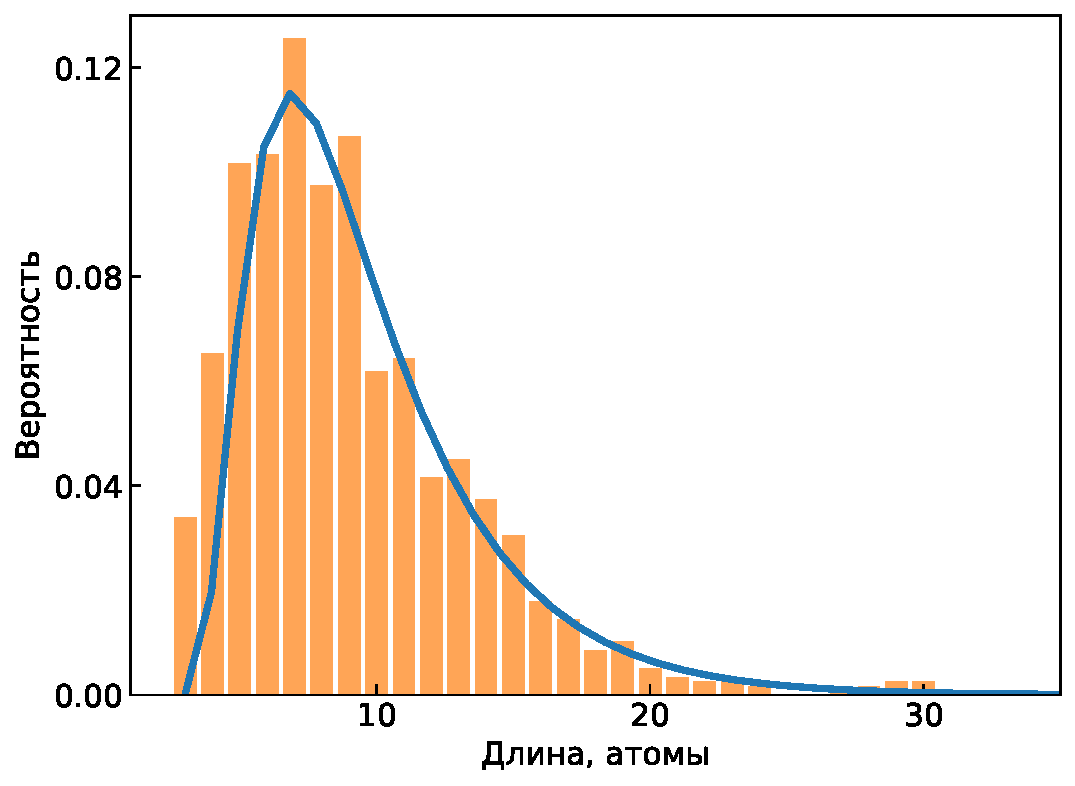
\includegraphics[width=0.65\linewidth]{fig/eqnoneq/fig4-ExpVsTheor.pdf}
	\caption{Гистограмма: экспериментальное распределение размеров одномерных островков Ag на вицинальной поверхности Pt(997)~\cite{PhysRevB.73.245425}. Линией показано неравновесное распределение длин островков согласно~\eqref{NonEqDistr} при $K=430$ и наиболее вероятной длине островка $l_{mp}=7$.}
	\label{fig:ExpVsTheor}
\end{figure}

Четвертый параграф посвящен вопросу определения энергии связи в одномерных островках. Обсуждается время жизни островков в контексте продолжительности эксперимента. Приводится алгоритм определения энергии связи из экспериментальных данных.


\textbf{Шестая глава} посвящена структурному фазовому переходу в одноатомной цепочке атомов кобальта на вицинальной поверхности меди.

В первом параграфе предложена модель, позволяющая изучить структурный фазовый переход в цепочке кобальта из димеризованного состояния в недимеризованное, ранее впервые наблюдавшийся экспериментально. Этот процесс был исследован при помощи алгоритма Метрополиса, энергетические барьеры для которого были получены из первопринципных расчетов. Кроме того, было показано, что в рамках теории функционала плотности возможно описать димеризованную структуру цепочки кобальта, вопреки заключению, сделанному в работе~\cite{PhysRevB.89.205427}.
Второй параграф посвящен влиянию различных параметров, таких как температура и длина цепочки, на критическую температуру структурного фазового перехода. Было показано, что критическая температура может изменяться в том числе и благодаря наличию над цепочкой иглы сканирующего туннельного микроскопа. Обсуждается размерный эффект. Показано, что критическая температура линейно растет вместе с $1/\ln N$, где $N$ --- длина цепочки.

\chapter{Основные результаты и выводы}
\begin{enumerate}
	\item С использованием теории функционала электронной плотности и метода Монте-Карло развита методика, позволяющая моделировать и исследовать формирование и эволюцию морфологии одномерных  металлических структур на вицинальных металлических поверхностях в зависимости от различных параметров эксперимента, а также исследовать структурный фазовый переход в них.

	\item Исследовано взаимодействие адатомов $3d$-металлов со ступенью вицинальной поверхности меди и объяснена их природа. Показано, что взаимодействие между двумя адатомами $3d$-металлов на вицинальной поверхности меди существенно зависит от расстояния до ступени.

	\item Выявлены основные факторы, влияющие на рост одномерных атомных металлических структур на вицинальных металлических поверхностях. Исследованы основные этапы формирования одномерных атомных металлических структур кобальта на вицинальной поверхности меди как в однотемпературном, так и в двухтемпературном режимах.

	\item Показано, как форма распределения длин атомных цепочек на вицинальных металлических поверхностях, а также положение его максимума зависит от ширины террас поверхности, степени покрытия, потока осаждаемых атомов и температуры.

	\item Была предложена модель для описания распределения одномерных атомных структур, в которой были учтены такие явления, как созревание Оствальда и распад коротких одномерных структур. В рамках этой модели предложен метод более точного определения значения энергии связи.

	\item В системе Co/Cu(775) обнаружено наличие двух структурных фаз для  атомных цепочек кобальта. Определена зависимость температуры структурного фазового перехода от длины цепочки и от энергии димеризации.
\end{enumerate}


\titleformat{\section}[display]{\centering\normalsize\itshape}{}{1em minus 1em}{}[]
\titlespacing{\section}{0cm}{*0}{*2}

\chapter{Список публикаций по теме диссертации}

\begin{refsection}
	\nocite{%
		Syromyatnikov:jetp-letters-rus:2014,
		Syromyatnikov:mplb:2016,
		Syromyatnikov:matlet:2016,
		Syromyatnikov:jetp-rus:2017,
		Syromyatnikov:PhysRevB:2018,
		Syromyatnikov:jetp-letters-rus:2018,
		SyromyatnikovJetpl2019rus,
		SyromyatnikovMagLett2019,
		Syromyatnikov2020SurfSci,
		Syro-JMMM-2020}

	\section{Публикации в рецензируемых научных изданиях, индексируемых в базах данных Web of Science и SCOPUS}
	\printbibliography[heading={none},resetnumbers=true]
\end{refsection}

\begin{refsection}
	\nocite{%
		Syromyatnikov:ECOSS30,
		Syromyatnikov:Lomo-rus:2015,
		Syromyatnikov:ECOSS32,
		Syromyatnikov:Lomo-rus:2016,
		Syromyatnikov:CHPH-WI:2017,
		Syromyatnikov:ICNT:2018,
		Syromyatnikov:CHPH-WI:2018,
		Syromyatnikov2019IBCM,
		klavsyuk2019IBCM,
		Klavsyuk2019IWMW,
		Syromyatnikov:CHPH-WI:2020}

	\section{Иные публикации (статьи в сборниках материалов конференций)}
	\printbibliography[heading={none},resetnumbers=true]
\end{refsection}

%\clearpage
\vspace*{1.5cm}

\printbibliography
\addcontentsline{toc}{chapter}{\bibname} % yes, after \printbibliography

\vfill\hfill{\tiny \textcolor{black!20!white}{\texttt{\GitDescribe}}}

\end{document}
